%% The following is a directive for TeXShop to indicate the main file
%!TEX root = ../MJThesis.tex
\acresetall

\chapter{Introduction}
\label{ch:Introduction}

\begin{epigraph}
    \emph{But during the writing of this review, I learned how little I knew in this area, and this was a humbling and sobering experience. I am certain that I have made many mistakes due to my ignorance, and I hope that the review will be useful despite its many faults} ---~Hiroshi Nikaido (2003), my grand supervisor.
\end{epigraph}

\section{Paracrystalline protein surface layers} % (fold)
\label{sec:paracrystalline_protein_surface_layers}

    \subsection{S-layer structure} % (fold)
    \label{sub:s_layer_structure}

        % \begin{comment}  % Notes on structure
        %         Notes on structure of S-layers:
        %             - Location (ref fig)
        %                 - anchor
        %             - Visual appearance 
        %                 - symmetry patterns (ref fig)
        %             - Protein vs glycoprotein
        %                 - protein specifics
        %             - Sequence gazing
        % \end{comment}

        \begin{figure}[p] % Cell envelopes diagrams
                \begin{center}
                    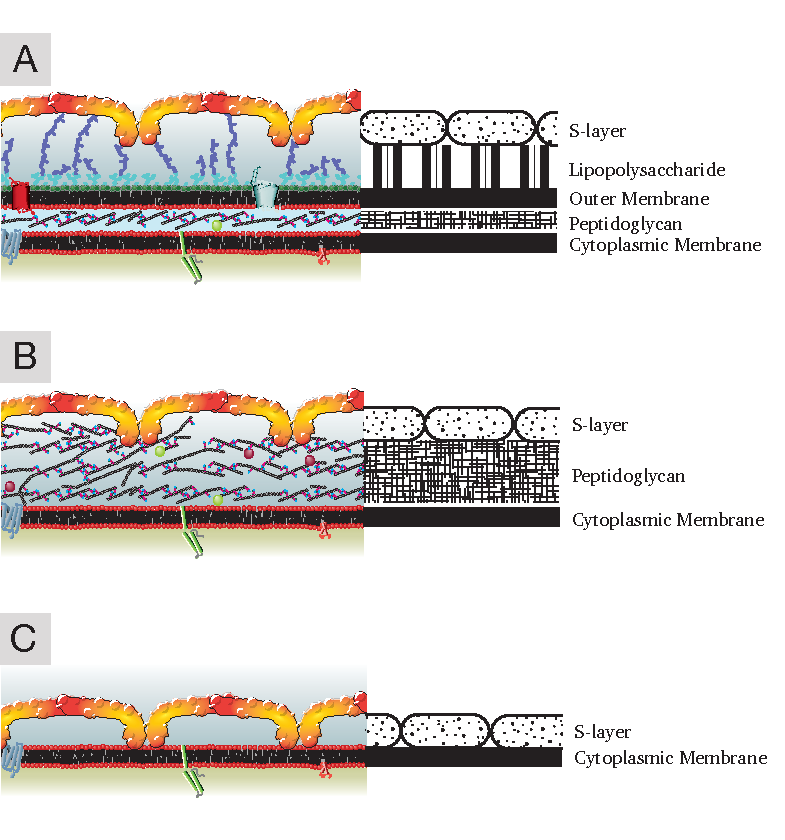
\includegraphics[]{intro/img/celwalls.pdf}
                \end{center}
                \caption[Cross-sectional diagrams of the cell envelopes]{Cross-sectional diagrams of the cell envelopes of (\textbf{A}) Gram negative bacteria, (\textbf{B}) Gram positive bacteria, and (\textbf{C}) archaebacteria. In all known cases the \ac{S-layer} sits on the extreme outer surface of the cell. (This diagram was inspired by Fig. 1 from \fullcite{sleytr1983crystalline})}
                \label{fig:cellwalls}
        \end{figure}

        \begin{figure}[htb] % S-layer
            \begin{center}
                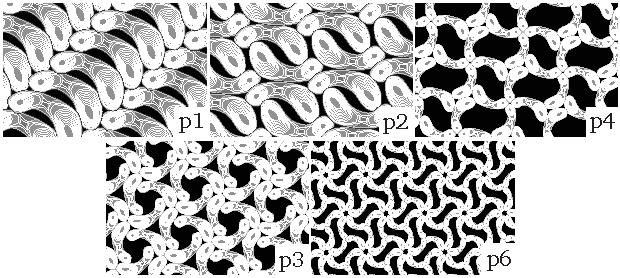
\includegraphics[]{intro/img/symmetries.pdf}
            \end{center}
            \caption[A simple overview of \ac{S-layer} symmetries]{A simple overview of \ac{S-layer} symmetries. p1 and p2 are oblique symmetries. Examples of bacteria with oblique \acs{S-layer} are \textit{Bacillus stearothermophilus} NRS2004$/$3a\upcite{messner1986characterization} and \textit{Lactobacillus brevis}\upcite[.]{masuda1980reassembly}
            p4 is a rectangular symmetry.  Examples of bacteria with rectangular \acs{S-layer} are \textit{Corynebacterium diphtheriae}\upcite{kawata1972extracellular} and \textit{Aeromonas salmonicidae} A450\upcite[.
            ]{ishiguro1981loss}
            p3 and p6 are triagonal$/$hexagonal symmetries.  Examples of bacteria with triagonal$/$hexagonal \acs{S-layer} are \textit{Bacillus anthracis}\upcite{holt1969comparative} and \caulobacter\upcite[.]{smit1981periodic}
            }
            \label{fig:symmetries}
        \end{figure}
    % subsection s_layer_structure (end)

    \subsection{History of S-layers} % (fold)
    \label{sub:history_of_s_layers}
       
       % \begin{comment}  % Notes on history
       %      Notes on history of S-layers:
       %          - first seen
       %          - first cloned
       %          - first crystallised

       %      First (always) seen by EM

       %      First seen in Spirillum
       % \end{comment}

        \begin{figure}[p] % First S-layer
                \begin{center}
                    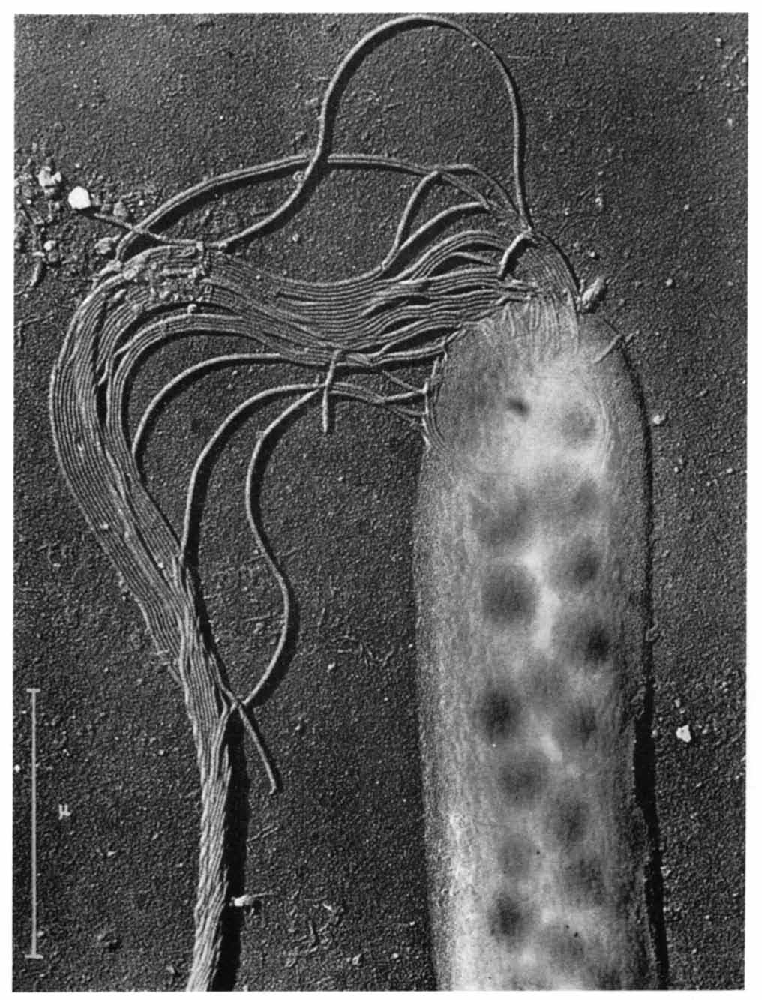
\includegraphics[]{intro/img/firstslayer.pdf}
                \end{center}
                \caption[The first published image of a \ac{S-layer}]{The first published image of a \ac{S-layer}. The hexagonal \ac{S-layer} on the surface of the bacterium --- probably \textit{Spirillum} sp. --- is visible along the edges of the cell body (centre right). The scale bar denotes one micrometre. (This image is Fig. 1 from \fullcite{firstslayer}, reused with full permission from the publisher, Elsevier.)}
                \label{fig:firstslayer}
        \end{figure}
    % section history_of_s_layers (end)
% section paracrystalline_protein_surface_layers (end)

\endinput

Any text after an \endinput is ignored.
You could put scraps here or things in progress.
